\section{Problema 6 - Contagem de números primos}

O problema pede para se contar quantos números primos são encontrados dentro do intervalo N, usando a distribuição cíclica e em blocos. A distribuição em blocos sobrecarrega o último processo pois passa para ele os maiores números, que demoram mais para serem testados, enquanto a distribuição cíclica distribui os números de forma mais uniforme entre os processos.

A decomposição cíclica sugerida pelo problema, apesar de distribuir os números de forma homogênea, não é adequada para o problema, pois ela ainda sobrecarrega os processos de rank ímpar, visto que esses recebem os números ímpares. 

Os processos que recebem os números pares param de executar na primeira linha de teste(a divisão por 2), por isso a decomposição cíclica utilizada para se obter os resultados dessa seção foi feita da seguinte forma:

P0 -> 3, 11, 19, 27, ...

P1 -> 5, 13, 21, 29, ...

P2 -> 7, 15, 23, 31, ...

P3 -> 9, 17, 25, 33, ...

usando-se de um laço for i in range(3 + rank*2, N, size*2):

Mediu-se o tempo de execução com a função MPI\_Wtime()(\citeonline{mpidoc}) para $N = 10^3, 10^4, 10^5, 10^6 e 10^7$, variando o número de processos entre 1, 2, 4 e 6. Com esses dados, calculou-se a Speed up e a Eficiência, que foram plotadas nos gráficos abaixo.

\begin{figure}[H]
    \centering
    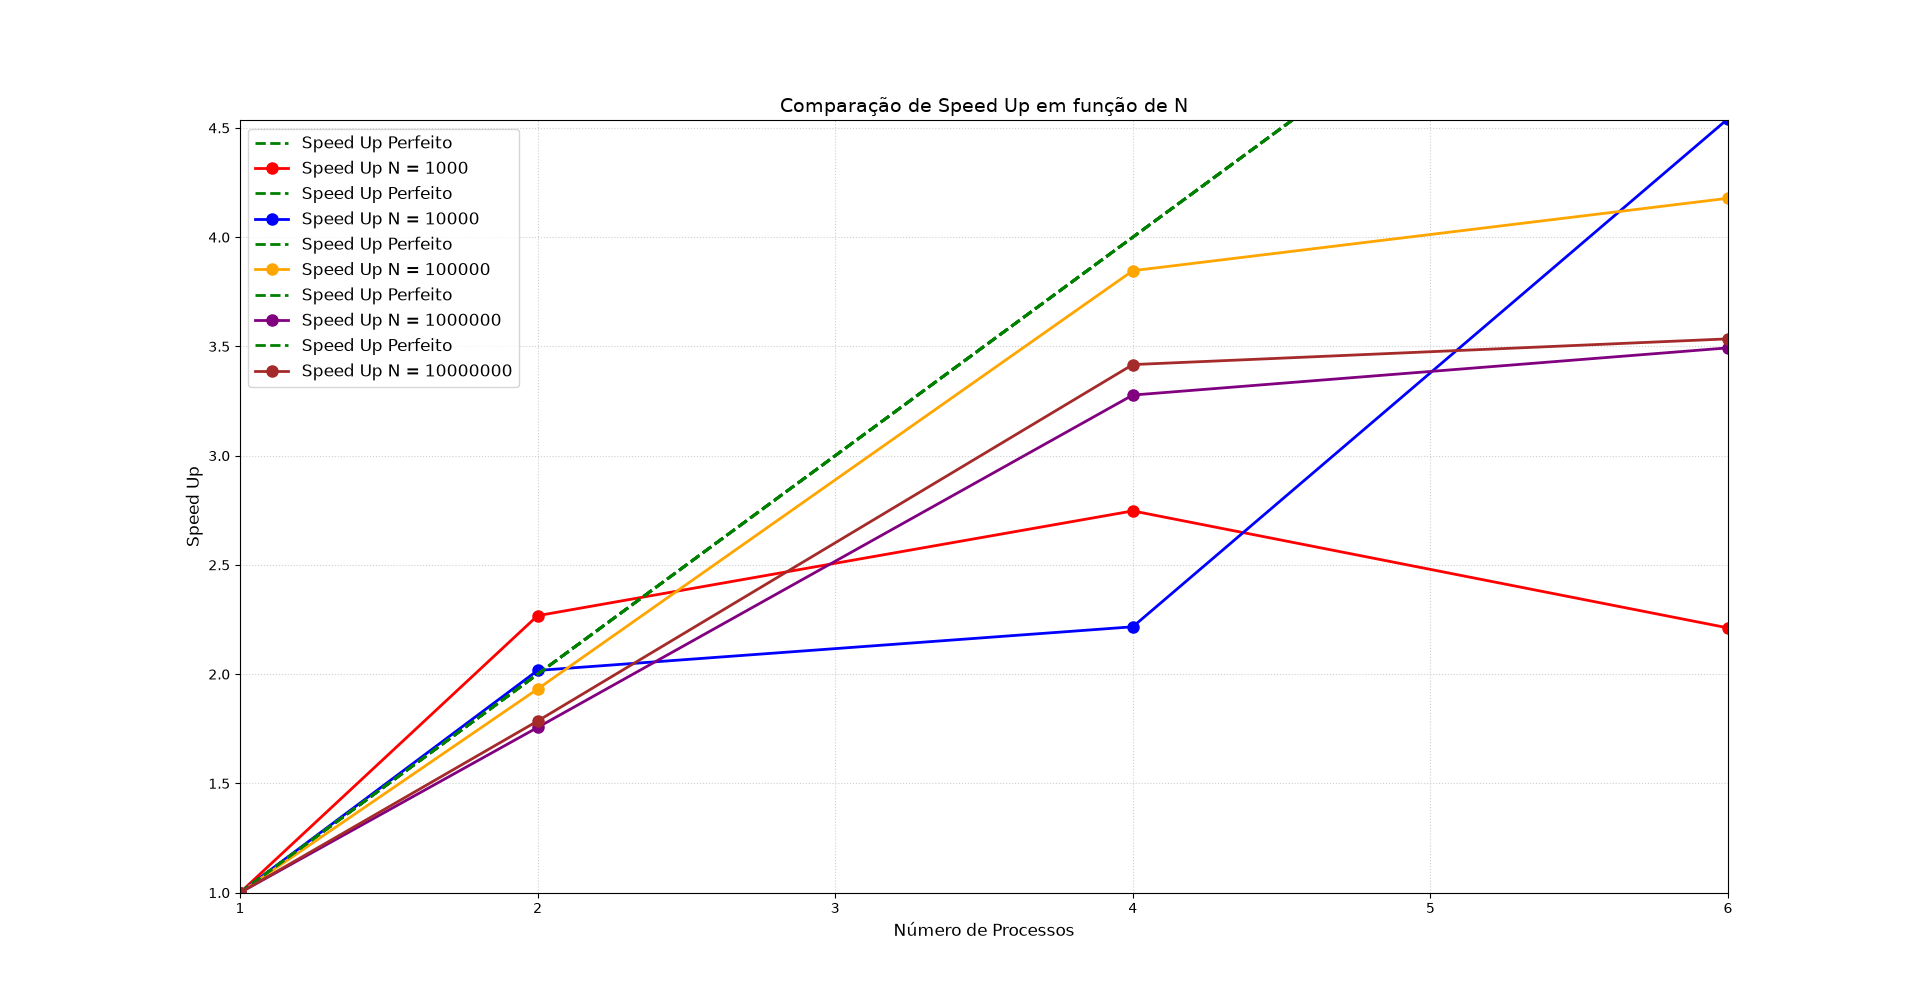
\includegraphics[width=1.2\textwidth]{figuras/primos_speed_up.png}
    \caption{SpeedUp para diferentes valores de N e número de processos.}
    \label{fig:primos_efficiency}
\end{figure}

\begin{figure}[H]
    \centering
    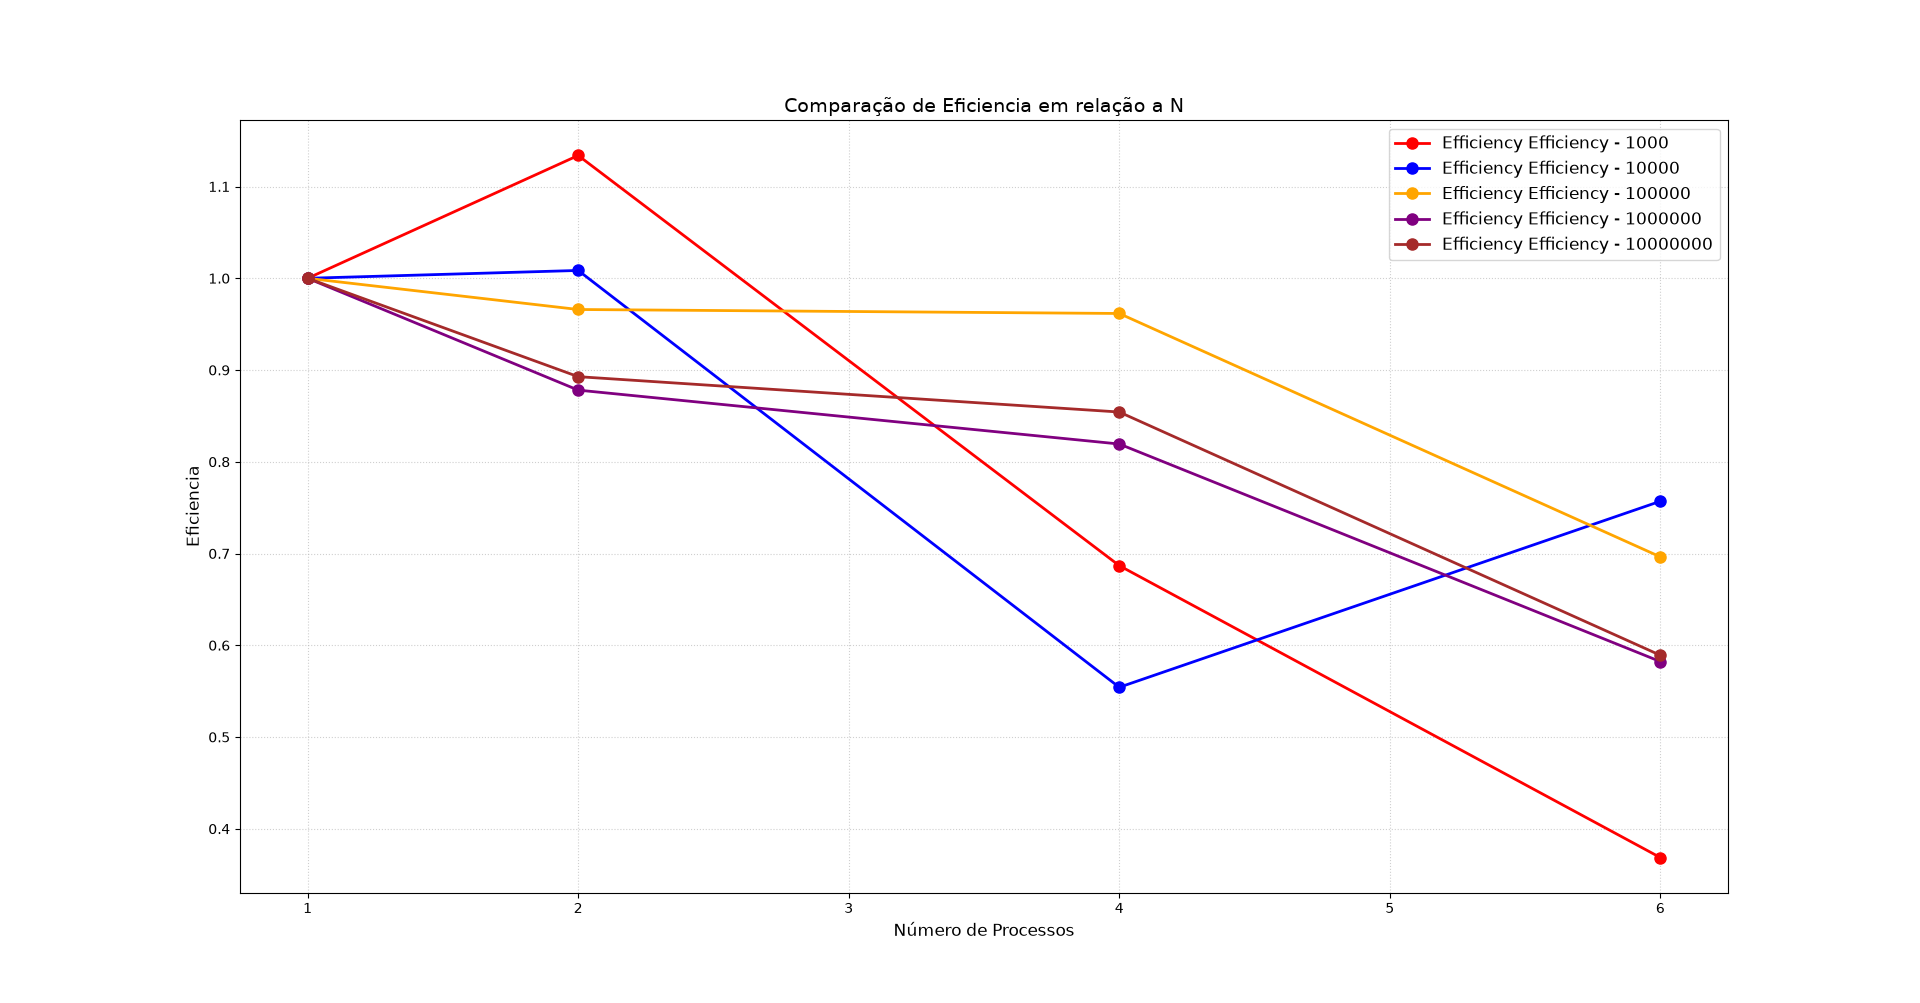
\includegraphics[width=1.2\textwidth]{figuras/primos_efficiency.png}
    \caption{Eficiência para diferentes valores de N e número de processos.}
    \label{fig:primos_efficiency}
\end{figure}


Quanto maior o número de números a serem testados, maior o tempo de execução, pois quanto maior o número a ser testado, mais tempo ele leva para ser testado. A distribuição foi feita de forma cíclica, ou seja, a distribuição está homogênea, logo nenhum processo está sobrecarregado. 

Para a fase de broadcast e scater, como os elementos são alocados localmente, o custo de comunicação é irrelevante, visto que o único elemento compartilhado é o número total de números a serem testados(não o vetor contendo esses números). 

Para a fase de gather, o custo representa a necessidade de cada processo enviar a lista com os números primos por ele encontrados, como a divisão é homogênea, em tese essa lista tem tamanho similar, logo o custo de comunicação deve ser mais ou menos constante.

Cada processo é criado uma única vez e eles devem apenas retornar a lista de números primos, que pode ser obtida com um gather e não há necessidade de sincronização, visto que cada processo é independente e não há necessidade de esperar por outros processos, pois eles só buscam por primos dentro do intervalo que lhes foi atribuído.

Observando as curvas, nota-se que a partir de N = 100 000 o speed up apresenta um comportamento semelhante para os demais valores de N, onde até 4 processos o crescimento é quase igual ao perfeito, mas para o processo 6 ele começa a cair. A eficiência também cai de forma quase que constante. Por conta desse comportamento semelhante, conclui-se que a partir de N = 100 000 começa a valer a pena paralelizar com pelo menos 4 processos.
